\chapter{Integration of structured biological data sources using Biological Expression Language}
\label{ch:bio2bel}

\section*{Preface}

Following the knowledge graph enrichment workflow presented in Chapter~\ref{ch:recuration}, the following paper describes the development and application of the \ac{BEL} a medium for integrating heterogeneous, multi-scale, and multi-modal structured biological data sources.
Towards this end, numerous independent \textit{Bio2BEL packages} have been developed capable of downloading, structuring, and serializing various biological data sources to \ac{BEL} as well as an overarching computational framework so that other software developers and biological data source owners can contribute their own Bio2BEL packages.
The philosophy of Bio2BEL encourages reproducibility, accessibility, and democratization of biological data sources.
The inclusion of numerous authors across several institutions shows the potential of the Bio2BEL philosophy as well as realizes the goals from Chapter~\ref{ch:pybel} to make the PyBEL ecosystem usable by others.

\vspace*{\fill}

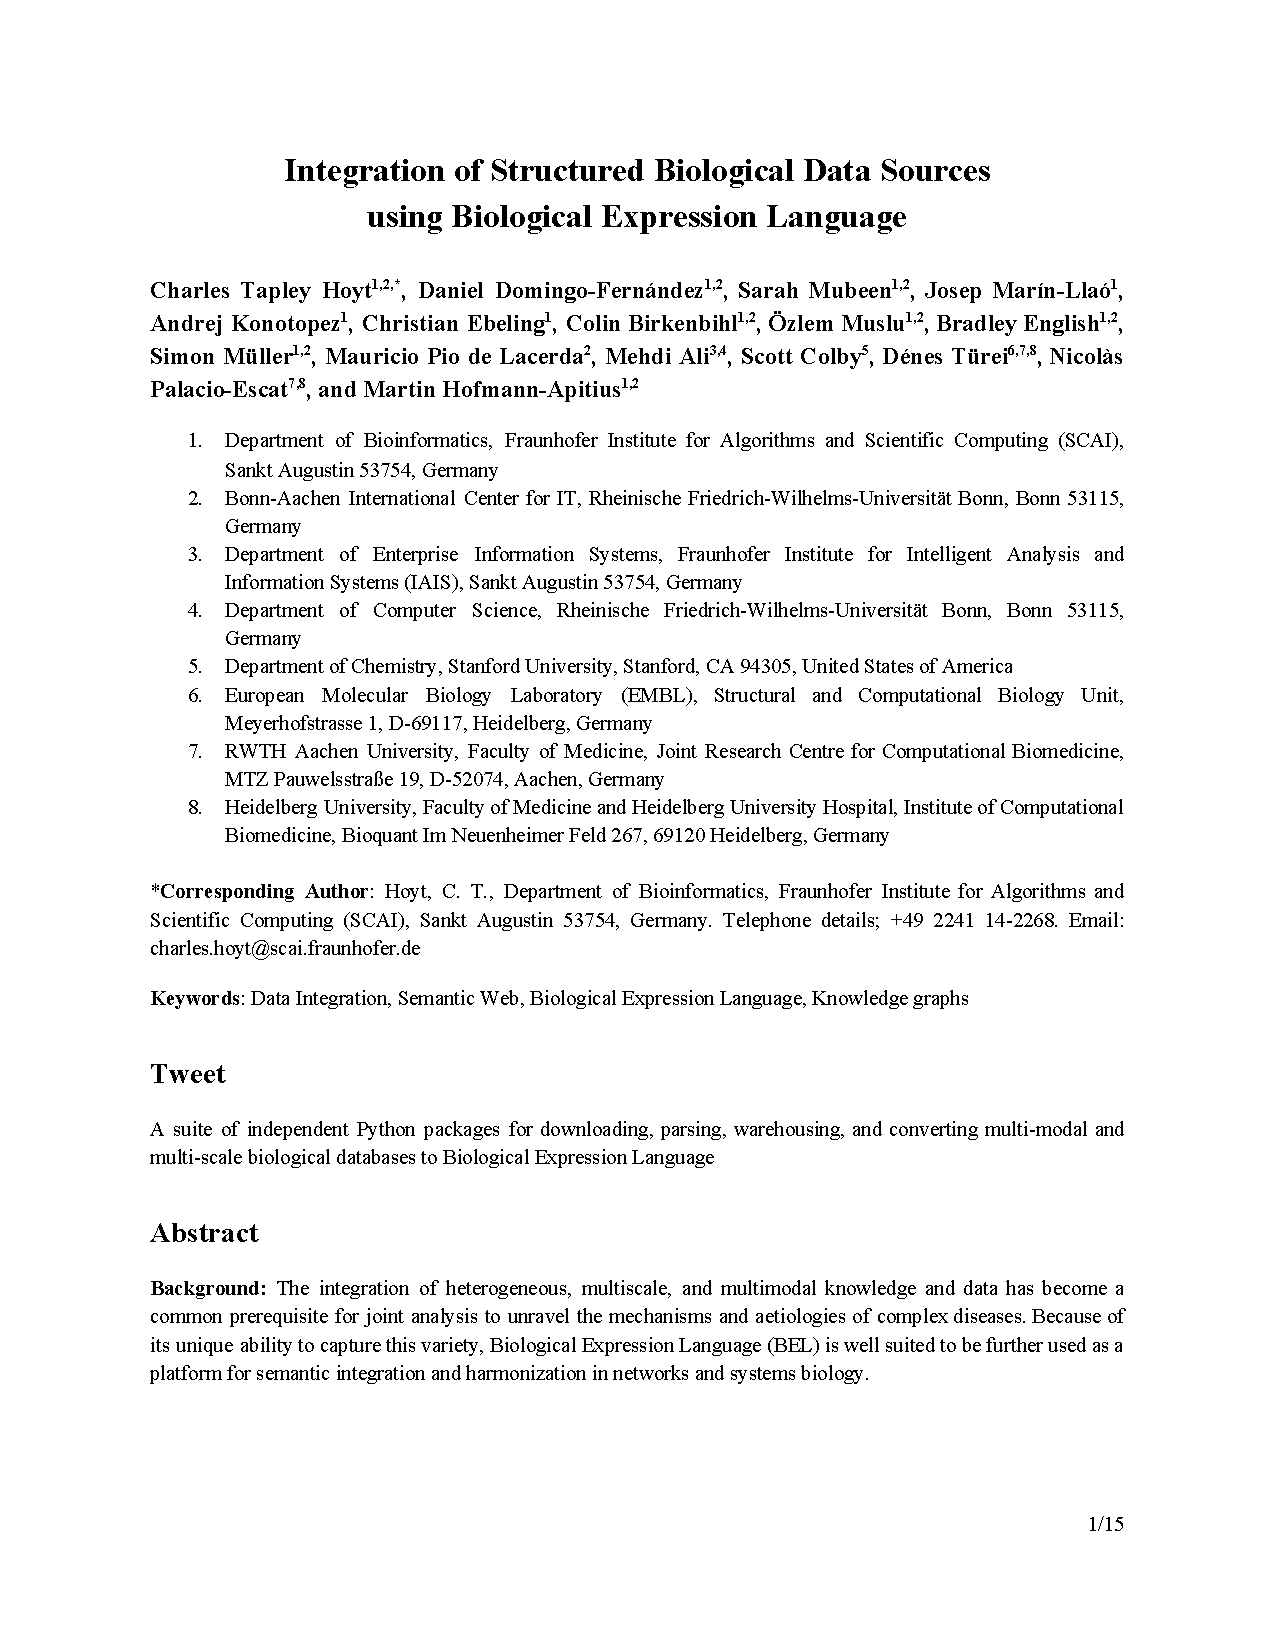
\includepdf[pages={-}]{articles/bio2bel.pdf}

\section*{Postface}

Several applications of Bio2BEL were presented: 1) the mapping of pathways between databases like \ac{KEGG}~\cite{Kanehisa2017}, Reactome~\cite{Fabregat2016}, and WikiPathways~\cite{Slenter2018} for the ComPath database~\cite{Domingo-Fernandez2018}; 2) the harmonization of pathway databases into a common schema using PathMe~\cite{Domingo-Fernandez2019a}; the application of network representation learning methods using BioKEEN~\cite{Ali2019}, and the integration with several other data aggregation systems like \ac{INDRA}~\cite{Gyori2017} and OmniPath~\cite{Turei2016}.
Given the PyBEL ecosystem first introduced in Chapter~\ref{ch:pybel}, the environment for exploration presented in Chapter~\ref{ch:belcommons}, the enrichment workflow presented in Chapter~\ref{ch:recuration}, and Bio2BEL, it is possible to generate and handle high quality biological knowledge graphs to support downstream analysis.
The remaining Chapters~\ref{ch:bel2abm},~\ref{ch:guiltytargets}, and~\ref{ch:epicom} constitue three examples of these downstream analyses.
